% 1962 年全国卷第 5 题：圆外切平行四边形为菱形。
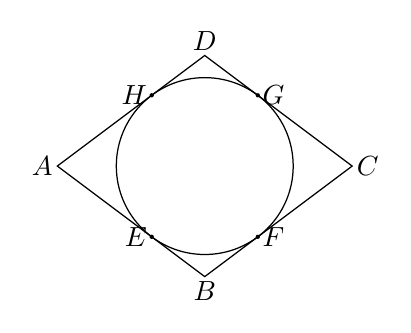
\begin{tikzpicture}[scale=0.78, line width=0.45pt,
  every node/.style={inner sep=1.5pt}]
  \coordinate (A) at (-2.4,0);
  \coordinate (B) at (0,-1.8);
  \coordinate (C) at (2.4,0);
  \coordinate (D) at (0,1.8);
  \coordinate (E) at (-0.864,-1.152);
  \coordinate (F) at (0.864,-1.152);
  \coordinate (G) at (0.864,1.152);
  \coordinate (H) at (-0.864,1.152);
  \draw (0,0) circle (1.44);
  \draw (A)--(B)--(C)--(D)--cycle;
  \fill (E) circle (0.035) (F) circle (0.035) (G) circle (0.035) (H) circle (0.035);
  \node[anchor=east] at (A) {$A$};
  \node[anchor=north] at (B) {$B$};
  \node[anchor=west] at (C) {$C$};
  \node[anchor=south] at (D) {$D$};
  \node[anchor=east] at (E) {$E$};
  \node[anchor=west] at (F) {$F$};
  \node[anchor=west] at (G) {$G$};
  \node[anchor=east] at (H) {$H$};
\end{tikzpicture}
